\documentclass{ctuthesis}
\usepackage[ruled,vlined,linesnumbered]{algorithm2e}

\ctusetup{
    xdoctype = B,
    xfaculty = F3,
    mainlanguage = english,
    titlelanguage = english,
    title-english = {Expedition scheduling in an automated warehouse},
    title-czech = {Rozvrhování vyskladňování z automatizovaného skladu},
    specification-file = {zav_prace.pdf},
    front-specification = true,
    department-english = {Department of Computer Science},
    author = {Jan Kalina},
    supervisor = {Ing. Martin Schaefer},
    supervisor-address = {Unknown,\\ Zářivá 232,\\
      12000 Praha 2},
      day = 13,
    month = 5,
    year = 2019,
    keywords-english = {scheduling, automated warehouse, optimization, simulation},
}

\ctuprocess

\begin{thanks}

TBD
\end{thanks}

\begin{declaration}

Prohlašuji, že jsem předloženou práci vypracoval
samostatně a že jsem uvedl veškeré použité informační zdroje v souladu
s Metodickým pokynem o dodržování etických principů při přípravě vysokoškolských
závěrečných prací.
\medskip


V Praze, \ctufield{day}.~\monthinlanguage{second}~\ctufield{year}

\end{declaration}
\begin{abstract-english}
This thesis deals with the optimization problem of expedition scheduling in an automated warehouse with a given set of parameters, requirements and set of items to dispatch in a day. Relevant scheduling problems and their solutions are discussed. Optimization method and objectives are then proposed for the given type of an automated warehouse. The proposed method is implemented in the provided simulation tool and evaluated based on its performance in the simulation.

\end{abstract-english}



\begin{abstract-czech}
test \ldots
\end{abstract-czech} 

\begin{document}

\maketitle

\chapter{Introduction}

Scheduling is a well studied and practical topic. It is widely used in manufacturing facilities, warehouses, which are discussed in this thesis, and many other industries where proper scheduling can play a great role in their success. Despite its importance and years of research, scheduling is quite a challenging problem, especially when it comes to real-world problems where finding an optimal schedule is usually nearly impossible due to its high computational complexity. 

Since the beginning of research in scheduling, many methods and approaches were developed for finding schedules close to optimal schedule in a reasonable time, but what is a good or optimal schedule? Determining the objective of a schedule is a problem on its own. The usual objective of scheduling is to minimize the makespan, which is the duration of a schedule. This objective alone is usually not sufficient because it does not consider the stochastic nature of real-world, where random events can change the schedule for the worse. In that case, the most valuable schedule might be the one where these random events change a schedule the least, and makespan is still small. Another reason why makespan or other simple objectives that are often mentioned in literature might not be sufficient is that some facilities may demand complex customized requirements tailored just for them. For example, in case of an automated warehouse, it may be crucial to not only finish expedition in required time but to also expedite items in the required order. 

In this thesis, general methods for solving scheduling problems relevant to scheduling a daily expedition of the given automated warehouse configuration are discussed. Then, method and an objective of a schedule for the given automated warehouse and scenario is proposed. Finally, the proposed method is implemented and evaluated in the simulation.

\section{The automated warehouse}
\label{sec:wh}
There are many different types of automated warehouses with very different requirements, structures, and functionality. The problem of scheduling an expedition can be very different based on the structure and the type of an automated warehouse. The basic structure and functionality of an automated warehouse based on a real-world problem were provided for this thesis and can be described as follows.

\subsection{Description}
\label{subsec:Description}
The automated warehouse is part of a factory. The factory stores products to the automated warehouse from which they are at some point expedited. Firstly, we describe production together with the automated warehouse and secondly, we describe the expedition process.

\subsubsection{Production and the automated warehouse}

The factory produces up to thousands of items throughout a whole day. Items come in hundreds of different types, which may differ in size, material, or in other properties, which are not important for this thesis. Since the warehouse is automated, items must have suitable weight and size to be handled by a stacker crane and to be stored in high-bay racks. An example of such items is tires or pallets of different sodas. Produced items are directly put one-by-one on the conveyor leading to the warehouse, where an item is pushed off the conveyor to the production buffer of one of the aisles.

The automated warehouse has given a number of aisles. Each aisle has high-bay racks on both sides and is connected to two conveyors at the beginning of it. The first conveyor is moving items from an aisle to a conveyor junction and then one of the expedition ramps, and the second one is bringing in items from production. Each aisle has a single stacker crane operating on it.

Stacker cranes operate automatically and can either store an item from production if it is available or execute scheduled unloadings. 

If stacker crane is requested to unload an item, it moves to the position of an item, grabs it and moves to the beginning of an aisle, where it puts the item on the conveyor leading to an expedition ramp. In case of an item arriving from production to an aisle's production buffer. Stacker crane should retrieve this item from the production buffer and store in a free position in the aisle. If any production buffer overflows, production would have to be stopped, for that reason, stacker cranes prioritize storing an item over unloading. It means that as soon as a stacker crane finishes an operation in progress, it stores an item from production (if it is available at the buffer) even if it means delaying scheduled unloading.

\subsubsection{Daily expedition}
The expedition is spanned over a part of one day; we will further refer to this part as working hours. We are given information about when the working hours start and end. During the expedition, a truck can arrive at an expedition ramp at a scheduled time. Only one truck and be loaded at a time at each expedition ramp. There is also reserved time after which the next truck can arrive. Every truck requests a certain number of items of different types and order of these types in which they should be loaded into the truck for practical reasons. Which specific items will be expedited is known in advance and is expected that these items are distributed uniformly across all aisles. 

Before each item reaches an expedition ramp, it arrives at a conveyor junction and then proceeds to the expedition ramp's scanner, where it needs to be scanned. A scanner is located at the end of the conveyor before each expedition ramp. 

The order in which items they are processed by a scanner corresponds to order at which they are loaded into a truck. Scanners accept an item periodically. Since the scanner is processing items in the given interval, there has to be space between items on conveyor based on the speed of the conveyor and the duration of the interval. If too many items arrive too soon after each other, they pile up and may cause the conveyor to stop, which should never happen. To prevent stopping of a conveyor, there is a small buffer. A scanner also accepts an item as soon as possible. The number of items that pile up in the buffer during a daily expedition is one of the measurements of robustness to delays.

We also simplify our problem and assume that workers at the loading ramp can always pick up an item coming from the scanner. That means that scanners then create bottlenecks for each expedition ramp where throughput is limited by the frequency at which scanner can process items.

On top of all these specifications, it is expected that the expedition should not last longer than the working hours. Additionally, the duration of a truck expedition should not take too much time; there is constraint on how long the truck expedition should be. Parameters specifying these requests and the importance of these requests is something that a client should specify, and it has to be considered during the construction of a schedule.

\subsubsection{Available information}

Several basic parameters were provided for the given automated warehouse. These parameters include horizontal and vertical speeds and accelerations of stacker cranes, dimensions of a warehouse, speed and length of conveyors, duration of scanning an item, duration of grabbing an item from a conveyor, duration of putting an item on a conveyor and exact location of each item stored in the warehouse. For the expedition, we know count, types, and order at which items should be loaded for each truck. 

*add information about number of jobs, etc.. What should we expect

\begin{figure}
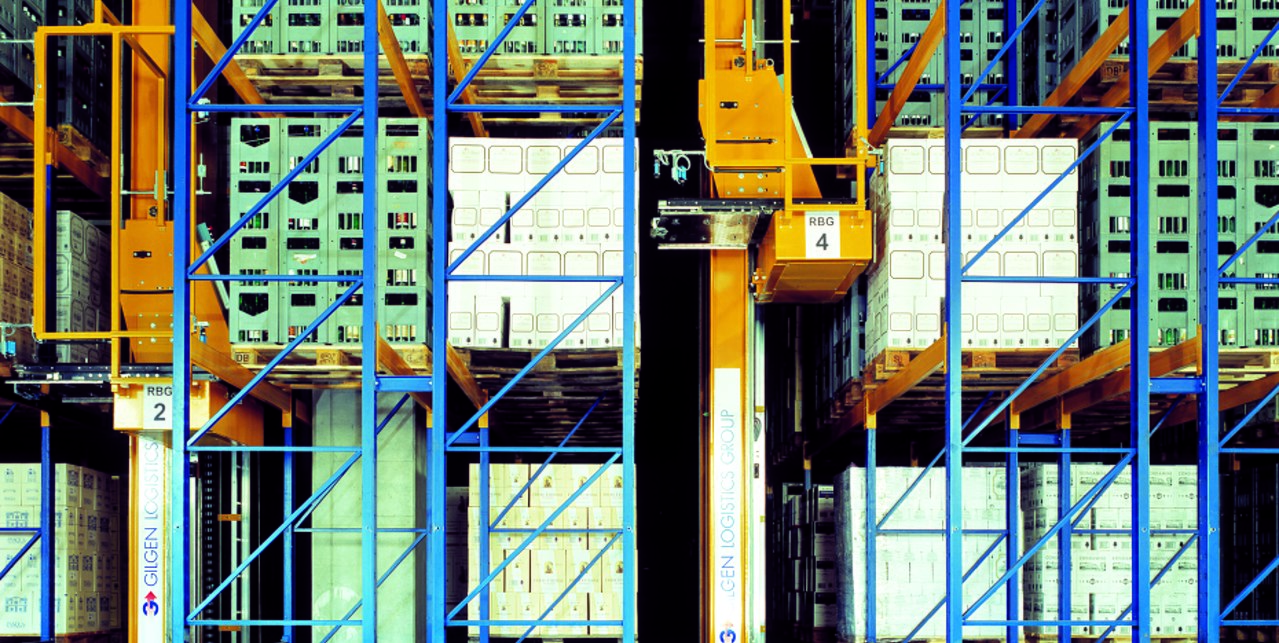
\includegraphics[width=0.8\linewidth]{highbaywarehouse.jpg}
\caption{Example of an automated warehouse with stacker cranes. \cite{warehousepic}}
\label{fig:foobar}
\end{figure}

\section{Goals and motivation}

The goal of this thesis is to create a schedule in a reasonable time by assigning trucks planned for a day to expedition ramps, determining their order and the order at which items will be expedited and finally determine the specific time at which stacker cranes should start unloading each item. Since there is no information about item production, we cannot incorporate production handling in our schedule, but knowing that production handling can delay an unloading of an item, we can try to minimize the effect that production handling has on the schedule. How much production handling affects the schedule, and if or how much are some of the requirements from Section \ref{sec:wh}, like preventing a buffer from filling up, violated sets how good the schedule is. To properly evaluate the schedule, it has to be integrated to provided simulation tool so that the created schedule can be observed in action and evaluated based on it. 

With a combination of the schedule and the simulation tool, we are also able to get data about the capabilities of the warehouse itself, which is valuable information when designing an automated warehouse. Integration of the scheduler to the simulation tool also enriches the simulation tool and can be used in future projects.

\section{Structure of this thesis}
*


\chapter{Problem statement}

\section{Notation and terminology}
in progress\\
\noindent \textbf{Job} ($job_i$) A $job_i$ represents an item $i$ to be expedited. Since expedition items are known in advance $job_i$ is already associated with one of the stacker cranes. 

\noindent \textbf{Machine} ($m_i$) A $m_i$ represents a stacker crane or a scanner. 

\noindent \textbf{Machine processing time} ($p_i$) Time which machine associated with $job_i$ needs to process $job_i$. In other words, the time needed to unload an item $i$ from its location to conveyor. This action consists of a trip from a conveyor to the item $i$, grabbing the item, trip back to the conveyor and putting the item on it. Values of $p_i$ are calculated from speeds, accelerations, and dimensions of the warehouse, but if production handling is taken into consideration, these values can become quite inaccurate since stacker crane may not always be at the same spot at the start of a job processing. Processing time is never zero.


\noindent \textbf{Scanning interval} ($s$) A processing time of a scanner in seconds. It is equal for every item and scanner.

\noindent \textbf{Traverse duration} ($t_i$) A time in seconds needed for an item to get from an aisle to a scanner by a conveyor.

\noindent \textbf{Completion time} ($c_i$) A time in second at a scanner finishes scanning of an item $i$.

\noindent \textbf{Idle time} ($\theta_i$) After processing an item $i$ at a scanner, the next item should be scheduled after the duration $\theta_i$ * lip to rict

\noindent \textbf{Assigned ramp} ($r_i$) An id of a ramp to which an item $i$ will be send to.

\noindent \textbf{Position in expedition} ($pos_i$ Position of an item $i$ in the expedition order. This number is determined by the time an item leaves the warehouse (reaches the conveyor junction)

\noindent \textbf{Set of ramp ids} ($R$) 

\noindent \textbf{Completion time of a truck} ($ct_i$) Time at which the last item of a truck arrives at its expedition ramp.

\noindent \textbf{Start} ($start$) The beginning of working hours. From this time on, trucks can be scheduled to arrive.

\noindent \textbf{Start} ($end$) The end of working hours. Ideally, every truck should be expedited.

\noindent \textbf{Stacker crane completion time} ($scc_i$) A time at which stacker crane unloaded an item $i$ onto a conveyor.

\noindent \textbf{Stacker crane start time} ($scs_i$) A time at which stacker crane starts unloading an item from the warehouse.

\noindent \textbf{Makespan} The duration of a schedule

\noindent \textbf{Reserve} TBD

\noindent \textbf{Average flow time} TBD

\noindent \textbf{Total flow time} TBD

\noindent \textbf{TBD - $expedition_{i,j}$ list, ... } ($something_i$)


\section{Scheduling problem}
 
 The problem of expedition scheduling in the automated warehouse can be separated into two problems, trucks allocation and item dispatching. The first problem of truck allocation is dealing only with the assignment of ramps to trucks. There are no requirements or constraints regarding order at which trucks should arrive at each ramp.
 
 The second problem, item dispatching, occurs after the truck allocation, and it deals with determining which items should meet which requests from trucks and the assignment of completion times of item unloading. Since machines are predetermined, there is no need to select a machine which unloads an item. An item is already associated with a machine.
 
Both of these problems are described as machine models in the following sections, which are used in scheduling literature (See \cite{pinedo} or \cite{bucker} for an overview of machine models). More formal formulations for both of these problems are included in following sections.
 
 \subsection{Trucks allocation}
 \label{subsec:truckallocation}
This problem can be formulated as a parallel machine model.
 
 There are $r$ ramps in parallel and $t$ trucks planned for a day. Ramps can be interpreted as machines in parallel and jobs as the whole expedition of each truck. 
 
 Since each ramp includes only one scanner, which acts as a bottleneck in the warehouse, the objective of this problem is to distribute expedition among ramps uniformly to utilize these ramps. In other words, workers at each expedition ramp should ideally work the same hours and do the same amount of work. 
 

  The problem can be formulated as assignment problem as follows:
 
 \begin{equation}\label{eq:to}
\begin{aligned}
&\text{minimize}
&&\max(y_0, \ldots, y_r)
\end{aligned}
\end{equation}
\text{subject to}\\
\begin{equation} \label{eq:ta1}
\begin{aligned}
    & \sum_{i=0}^{n} x_{ij} = 1 && \text{for } j=0, \ldots, r\\
\end{aligned}
\end{equation}
\begin{equation} \label{eq:ta2}
\begin{aligned}
    & \sum_{i=0}^{t} {d_i} \cdot x_{ij} = y_j && \text{for } j=0, \ldots, r
\end{aligned}
\end{equation}
  
Where $x_{ij}$ is a binary decision variable, which detonates that the $i$th truck is scheduled on $j$th expedition ramp. By satisfying Equation \ref{eq:ta1} it is ensured that every truck is assigned to only one ramp. Equation \ref{eq:ta2} sets variable $y_i$ to duration of expedition on the expedition ramp $i$. By minimizing Function \ref{eq:to} we minimize makespan, which leads a good utilization of machines \cite{pinedo}.

 
\subsection{Item dispatching}*prejmenovat, uz pouzivam nazev job dispatching jako cast algoritmu co tohle resi
\label{subsec:expeditiondispatching}

The problem of assigning completion times to jobs in the automated warehouse can be formulated as a special case of 2-stage flexible flow shop (FF2) with blocking or flexible flow line (FFL) with two stages as follows:

There are two work stations connected in series. The first work stations consist of $m$ machines (stacker cranes) in parallel, and the second work station consists of $r$ machines (scanners) also in parallel. Every job $job_i$ needs to be processed on its predetermined machine, and processing of $job_i$ takes $p_i$ seconds. After job $job_i$ is processed, it travels $t_i$ seconds to get to a scanner where it needs to be processed too. Processing time $s$ of every scanner is the same. Jobs cannot wait between work stations. That alone is referred to as FFL.

Additionally, we need to ensure that an item $i$ arrives at a truck in an order at which this item's type is requested and since this problem follows the truck allocation problem, orders at which items should arrive at expedition ramp are known. By assigning an order and a ramp to an item from a warehouse, we assign an item to a request. This leads to the following problem formulation.

For convenience, we formulate this problem as constraint satisfaction problem as follows:

*Domeny promennych co nejsou soucasti pouze teto formulace popisu asi spis v notaci

\textbf{Variables:}
\begin{align}
    &V = \{c_{0}, c_{1}, \ldots, c_{n},r_0, \ldots, r_m, pos_0, \ldots, pos_n\}
\end{align}
\textbf{Domains:}
\begin{align}
&c_{i} \in C_i = \{start, ..., 86400\} && \text{for } i=0,\ldots,n\\
&r_{i} \in R && \text{for } i=0,\ldots,n\\
&pos_i \in \{1, \ldots, n\}
\end{align}
\textbf{Constraints:}
 \begin{align}
& pos_i < size_{r_i} && \text{for } i=0,\ldots,n \nonumber \\
& pos_i < pos_j \land r_i = r_j \implies c_i < c_j && \text{for } i=0,\ldots,n\\ \label{eq:idcons2}
& m_i = m_j \implies scc_i \leq scs_j \lor scc_j \leq scs_i && \text{for } i,j=0,\ldots,n\\ \label{eq:idcons1}
& r_i = r_j \implies c_i  + \theta_i \leq s_j \lor c_j + \theta_j \leq c_i - s && \text{for } i,j=0,\ldots,n\\ \label{eq:idcons4}
& expedition_{pos_i,r_i} = type_i  && \text{for } i=0,\ldots,n\\ \label{eq:idcons3}
\end{align}

Where constraint \ref{eq:idcons2} ensures that a variable $pos_i$ represent an order at which an item $i$ is loaded at expedition ramp $r_i$. Constraints \ref{eq:idcons1} and \ref{eq:idcons4} secures that stacker cranes and scanners can process only one item at a time respectively. Finally, Constraint \ref{eq:idcons3} checks if type of an item $i$ is expected at expedition ramp $r_i$ in $pos_i$-th order.

Main requirements of this problem are to make a schedule that fits into working hours of the warehouse and make the schedule robust to random events. For example, the arrival of an item from production can postpone scheduled job at a machine for a whole duration of storing the item, and that can lead to loading items in the wrong order and filling buffer at a scanner. 



\chapter{Related work}
\label{chap:Related work}
Methods for solving various forms of scheduling problems were extensively studied for decades now. Many of these methods are summarized in Scheduling by M. Pinedo \cite{pinedo} and Scheduling Algorithm by P. Brucker\cite{bucker}. We will mainly discuss methods from these books that apply to the flexible flow line or parallel machine model problems and some general methods, which are relevant for this thesis. 

\section{Overview of methods and approaches for finding optimal or nearly optimal schedule}

Both problems we consider in this thesis are NP-hard \cite{pinedo}. To find the optimal schedule of FFL or parallel machine model, seemingly two general methods are used, Mixed Integer Programming (MIP) and Constraint Programming (CP) with a combination of pruning methods, an approximation of initial bounds and other general methods. MIP approach is often obsolete for real-world problems, where there are hundreds or thousands of jobs to schedule. CP is in many cases similar to MIP, but offers better flexibility for designing constraints and can be optimized for specific problems and because of it often outperforms MIP. More on CP can be found in Principles of Constraint Programming by K. Apt \cite{cp}.

There are also some special cases of machine models and scheduling objectives for which we can construct an optimal schedule using different dispatching rules or algorithms. Neither FFL scheduling nor parallel machine model of truck allocation problem can be optimally solved using some dispatching rules as far as we know, but we will take a look on some special cases that can give as an idea what dispatching rules should perform well.

\section{General methods for solving scheduling problems in practice}

\subsection{Dispatching rules for parallel machine model and minimizing makespan}

There are few construction heuristics from which we can construct a schedule that guarantees an upper bound of the makespan \cite{gram}. One of these heuristics is The Longest Processing Time first (LPT) heuristics \cite{pinedo} that guarantees that \cite{gram1969}:

\begin{equation}
\dfrac{C_{max}(LPT)}{C_{max}(OPTIMAL)} \leq \dfrac{4}{3} - \dfrac{1}{3m}
\end{equation}

Where $m$ is a number of parallel machines.

But to find an optimal schedule, we need to use some general method like MIP or CP and LPT rule can be used for approximation of an upper bound.

\subsection{Dispatching rules for flexible flow line model}
\label{subsec:ffl}
To find an optimal schedule for FFL with even some basic objectives like makespan can be solved again by using some of the general methods like the CP. 

A rule that is worth mentioning is Johnson's rule (also known as SPT(1)-LPT(2)) for minimizing the makespan of FFL with two stages and a single machine at each of them. Johnson's rule constructs an optimal schedule by partitioning jobs into sets. The first set contains jobs that have processing time in the first stage lower than processing time in the second stage and the second stage vice-versa. 
Jobs from the first set are scheduled first in increasing order of their processing time (SPT). After that, jobs from the second set are scheduled in decreasing order of their processing time (LPT). Jobs with equal processing time in both stages can be added to either of these two sets. More about Johnson's rule can be found again in Scheduling by M. Pinedo \cite{pinedo}.

In our problem of item expedition, the processing time at a scanner is always the same and is lower than processing time at a machine. This gives us an idea that SPT rule should utilize machines in FFL well. Guinet \cite{guinet} proposed a heuristic method based on Johnson's rule for FFL and made a comparison to SPT and LPT rules and surprisingly concluded that LPT heuristics gives good result for makespan minimization (as stated by Kia \cite{kia}).

\subsection{Local search techniques}

In addition to mentioned dispatching rules like SPT, LPT or Johnson's rule, and general approach like CP, other popular methods for solving scheduling problems are variations of local search techniques.

Local search is another very wide topic. In this thesis, we will describe the very basic idea behind local search algorithms. Again, detailed information and examples can be found in Scheduling by M. Pinedo \cite{pinedo}. 

The local search algorithm takes an existing schedule an tries to improve it by searching through his neighborhood. The neighborhood consists of schedules that are generated from the original schedule using some specific operation; we will be referring to it as move. The algorithm makes a step by evaluating schedules from a neighborhood and selecting new schedule from which it creates a new neighborhood and begins another step. There are many types of local search algorithms that usually differ in the way they select or reject the next move or how they create neighborhoods. 

The specific algorithms that are often mention in literature are tabu-search, simulated annealing, and genetic local search.

Local search methods also do not guarantee to find an optimal schedule.

\chapter{Proposed solution}
\label{ch:Proposed solution}

The proposed algorithm is designed in a way so that it is relatively simple and fast so that it can be easily applicable in practice and can be potentially used for frequent rescheduling as a reaction to some random events.

It consists of four different phases.

\begin{enumerate}
    \item Truck allocation
    \item Job dispatching
    \item Re-ordering
    \item Idle time insertion
\end{enumerate}

The proposed method does not try to utilize machines optimally. Finding an optimal schedule requires lots of computational power. Several MIP formulations have been proposed, and various branch and bound approaches have been developed for these problems, but still, only problems with around 50 jobs can be solved in reasonable time \cite{pinedo}. Furthermore, because of the production handling, the original schedule may be disrupted, and the value of finding an optimal schedule will be lost. 

That being said, in the first phase algorithm optimally distributes trucks to ramps and thus solves the problem of truck allocation (Subsection \ref{subsec:truckallocation}). In the second phase, however, heuristic construction is used to get a good schedule by solving item dispatching problem (Subsection \ref{subsec:itemdispatching}) in a relatively short time. The third phase is used to further improve on assignments, which were made in the second phase using local search algorithms. In the last phase, we insert idle times in between completion times $c_i$ to achieve good robustness to delays caused by prioritized production handling \cite{pinedo}. 

\begin{figure}[H]
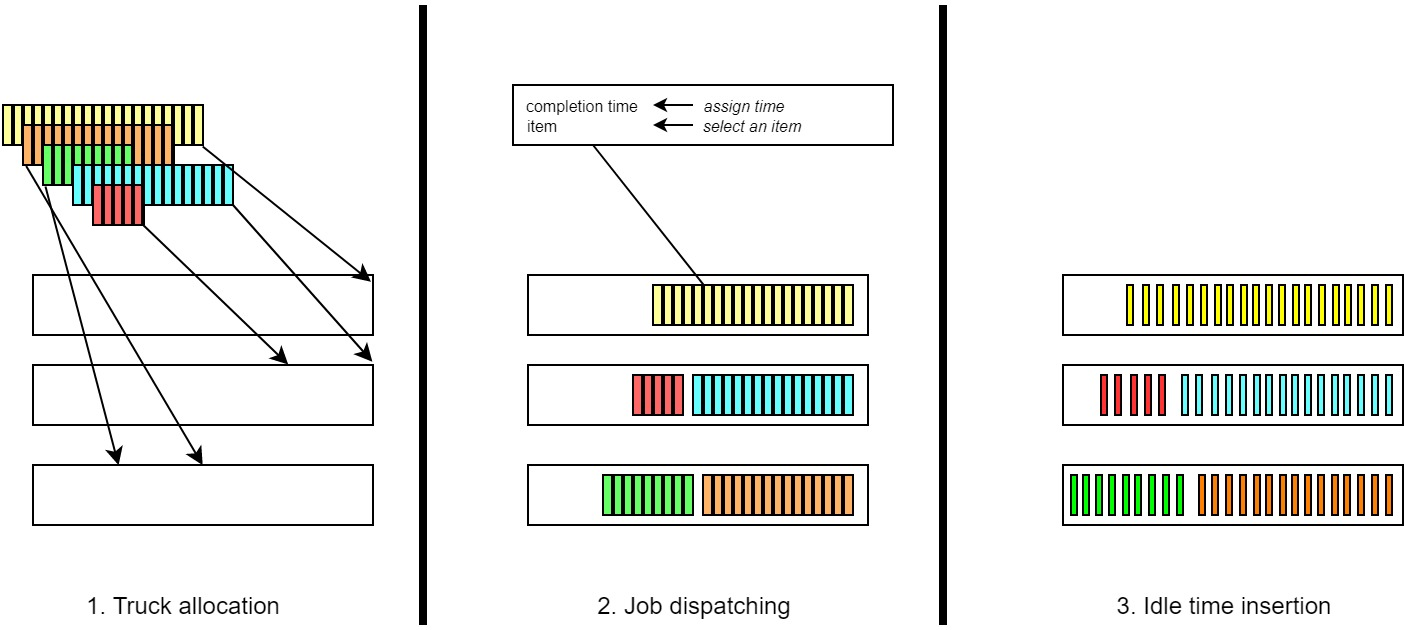
\includegraphics[width=1.0\linewidth]{algo.jpg}
\caption{Illustration of phases one to three of the algorithm.}
\end{figure}

\section{Score of the schedule}

To be able to compare different feasible schedules (See Subsection \ref{subsec:expeditiondispatching}), we introduce a score of a schedule. 

We formulate it as a sum of the weighted sub-objectives. The higher the score is, the better the schedule is.

Score:

\begin{equation}
\begin{aligned}
    &score = -\alpha T + \beta R - \gamma  U - \delta S && \alpha, \beta, \gamma, \delta > 0
\end{aligned}
\end{equation}

Sub-objectives:

\begin{enumerate}
\item \textbf{Maximum tardiness} $(T)$\\ \begin{equation}\max_{i=0,\ldots,n}(\max((c_i - end), 0)\end{equation}

The maximum tardiness represents the time by which the last item that arrived at the expedition ramp exceeded work hours. Ideally, the value of maximum tardiness is zero, meaning that the whole expedition fits into working hours.

\item \textbf{Sum of idle times} $(L)$\\ 
\begin{equation}
    \sum_{i=0}^{n} w_i \cdot \theta_i
\end{equation}

Maximizing the sum of idle times increases the robustness of the schedule (See \cite{pinedo}). Because one of the requirements is that items of the same type should be loaded in the given order, an expedited item that is followed by an item of a different type may benefit more from idle time. That is why we take weights of idle times into consideration.

\item \textbf{Constraint duration of truck expedition} $(U)$
\begin{equation} 
   U = \begin{cases}
        1 \text{ if } te_i - ts_i > maxdur_i\\
        \text{0 otherwise}\\
       \end{cases}
\end{equation}

This objective represents penalty for a truck expedition which takes too much time.

\item \textbf{Standard deviation of idle times} $(S)$
\begin{equation} 
    S^2=\frac{1}{n-1}\sum_{i=1}^{n} (\theta_{i} -\bar{\theta})^2 
\end{equation}

The goal of this objective is to keep idle times uniformly distributed. 

\end{enumerate}
 
 Experimenting with these objectives, weights, their effect and trade-off between them are shown in Chapter \ref{ch:Evaluation}.


\section{Truck allocation}
\label{sec:truckallocationprop}
In this phase, we solve the problem from Subsection \ref{subsec:truckallocation}. The goal of this phase is to distribute trucks among expedition ramps so that workers at each ramp work almost the same time and do nearly the same amount of work. This can be achieved by minimizing the makespan. By minimizing the makespan, we achieve good utilization of machines or in our case expedition ramps, which leads to a balanced load on expedition ramps \cite{pinedo}. 

In many factories as well as in the automated warehouse, there are not many trucks scheduled for a single day (under 50). On top of that, the objective of this problem, minimizing a makespan, is a very simple objective. This makes this problem a good example where CP or MIP performs well. Even for it being a real-world problem, finding the optimal solution for this case is valuable since stochastic events like "need to reschedule a truck to different ramp" or "truck needs more or fewer items than it originally demanded" do not occur very often.

This problem was already formulated as an assignment problem in Subsection \ref{subsec:truckallocation}. This formulation can be also used for the CP problem.

To improve the performance of these methods, we need to select \textbf{upper bound} of the objective and variables. Upper bound is calculated using LPT heuristics mentioned in Chapter \ref{chap:Related work}. Going back to the problem formulation in Subsection \ref{subsec:truckallocation}, we can not specify that the domain of the decision variables $y_i$ is $\{0, \ldots, C_{max}(LPT)\}$. The LPT heuristics can also be used as an alternative to CP or MIP solution for big instances of the problem.

There are no requirements for order at which trucks arrive, but assuming some trucks may be delayed. We propose ordering at which trucks arrive at the expedition ramp is determined by priority of a truck. A truck with higher priority is scheduled before a truck with lower priority on the same expedition ramp. If a truck is delayed, it affects trucks scheduled after it, and it creates a cascading effect, where all trucks behind the first delayed one are delayed if reserve time between them is not big enough.

The weights should be specified by a client, or assuming that trucks with bigger request have higher chance of getting delayed we order trucks in increasing order by size of a request.

\section{Job dispatching}

In this phase, we solve the problem from Subsection \ref{subsec:itemdispatching} and thus create a feasible schedule.
To obtain a feasible schedule, a constructive heuristic method is proposed. This method assigns values to variables in a way that after assigning value to every variable, we get a feasible solution without a need to backtrack.

In this phase, we also need to take into consideration some of the objectives. If machines are not utilized properly by the proposed method, the duration of the schedule might be greater than the duration of working hours or breakdown of a machine could have worse consequences. Also, items should arrive at different expedition ramps in similar rate to ensure that truck expedition does not take significantly longer than expected.
 
\begin{algorithm}[H]
\SetAlgoLined
\KwResult{A feasible schedule S}
  $items \leftarrow$ sort $items$\;
  \ForEach{$i$ in $items$}{
    $C_i \leftarrow$ sort in increasing order $C_i\;$
  }
 \For{$position \leftarrow 0$ \KwTo n}{
  $machines \leftarrow$ sort machines\;
  $ramp \leftarrow$ select a ramp\;
  \ForEach{$machine$ in $machines$}{
    \ForEach{$i$ in $items$}{
    \If{$m_i = machine$}{
    \ForEach{$time$ in $C_i$}{
    \If{$S \cup \text{\{i, time, ramp, position\} is feasible}$}{
    $pos_i \leftarrow$ position\;
    Add \{i, time, ramp\} to solution S\;
    $items \leftarrow items \setminus \{i\}$\;
    \textbf{goto} $mainLoopEnd$\;
}
}
}
}
}
[mainLoopEnd]\\
}
\caption{Job dispatching}
\end{algorithm}

The algorithm starts by putting items from the warehouse and times from domains $C_i$ to an ordered queue $items$ (See Subsubsection \ref{subsubsec:itemsordering}). Then algorithm selects a $ramp$ and cycles through $machines$ (stacker cranes) in established order until any $machine$ has an item with the same type as a request next in order on a $ramp$. Then it selects the shortest completion time from domain $C_i$ of an unload action of this item, that satisfy constraints from Subsection \ref{subsec:itemdispatching}. 


\subsubsection{Latest job last heuristic (Machines and ramp ordering)}

The aim of this heuristic is to get good utilization of machines at any time and process an expedition in all active ramps at similar speeds. The rule that is proposed to sort machines based on the time of the last processed unloading in increasing order and prioritize the first one. 
Basically, the same rule is proposed for the selection of an expedition ramp, but it is ordered based on the time that ramp's latest loaded item passed a conveyor junction (the time an item left the warehouse). Ordering by a time an item is loaded is not suitable, since travel time to different expedition ramps can be different, and thus it may result in different loading rates. *comparison in evaluation?

\subsubsection{Items ordering}
\label{subsubsec:itemsordering}

Items are ordered using LPT dispatching rule for reasons stated in Subsection \ref{subsec:ffl}.


\begin{figure}[h]
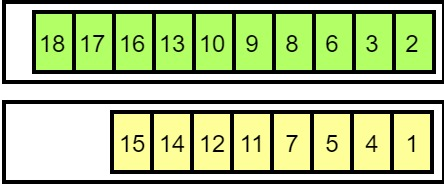
\includegraphics[width=1\linewidth]{order.jpg}
\caption{Diagram showing an ordering at which items are expedited.}
\label{order}
\end{figure}

\section{Re-ordering}

The goal of this phase of the algorithm is to improve the schedule by reordering items that were ordered using LPT heuristics in the second phase (See Subsubsection \ref{subsubsec:itemsordering}). The heuristics used in the second phase should create a good schedule, but it does not guarantee that the utilization of machines is optimal. This phase tries to bring it closer to the optimum.

The method that is proposed here is a local search algorithm (specific algorithms are compared in Chapter \ref{ch:Evaluation}. A move of a local search algorithm swaps order (See Subsubsection \ref{subsubsec:itemsordering}) of two items. After positions are swapped, the job dispatching algorithm must be run again, but items should be now sorted by their assigned position $pos_i$ and not by item ordering proposed in Subsubsection \ref{subsubsec:itemsordering}.

If we have a feasible schedule, the local search algorithm is a good alternative to the CP approach, or variants of a branch and bound, which do not perform well in problems of this scale. The local search ends after a certain amount of time or has no neighbour to select, and returns the best schedule that was found so far. This implies that step of the algorithm is optional, and in the worst case, we get the schedule from the second phase.

*obrazek

\section{Idle time insertion}

The goal of this phase is to take advantage of the remaining time of working hours, assuming there is remaining time, spread the expedition through the whole day and as a result create a more robust schedule. 

Since order at which items are expedited is one of the requirements (subsection \ref{expedition}), inserting idle times in between loading (or completion times) is crucial for minimizing number of errors in ordering due to delays caused by prioritized production handling. It also reduces the chance of scanner's buffer to overflow.


* misto toho, ze "item je asociovan s ..." Mozna bych mel rict, ze vytvarim tuhle asociaci a nebo to lip popsat na zacatku
Each scheduled item is associated with an idle time, which follows the arrival of the item to an expedition ramp. Other items cannot be scheduled to arrive after an item $i$ for its duration of idle time $\theta_i$.

*(to uz rikam u score)Idle times should be distributed uniformly to prevent scanner's buffer overflow, but some items that are followed by an item of a different type may benefit more from idle times, because it may also prevent disruption in an expedition order.

*odpoved na komentar*

The method that is proposed in this stage is step count hill climbing (SCHC) algorithm presented by Yuri Bykov \cite{yuri}. SCHC is based on hill climbing local search, but instead of finding the most valuable move across all moves, it first evaluates several moves and selects the one that improves the overall score of a schedule the most. The main benefit SCHC has over hill climbing algorithm or other some other local search algorithm is that we can set how many moves are evaluated in one step to regulate performance since job dispatching can be computationally demanding. To properly use SCHC, we have to specify what moves can this method use. 

There are $n$ moves, one for each item. Each move inserts some low amount of idle time (seconds) after arrival to an expedition ramp of an item. A move is part of a move list that is sorted in increasing order based on the size of idle time of an item that is associated with a move. SCHC evaluates several moves in this order and makes the next step; this continues until there are no improving moves to make or in other words, there is no remaining time left to distribute, or all truck expeditions reached their maximum allowed duration.

*pseudocode

In scenarios when there is a lot of time remaining (several hours) until the work hours end, idle time distribution may not perform well. To combat this performance issue, a special move is added to the beginning of the move list. This move inserts idle time to all items at once and thereby avoids unnecessary evaluations after every idle time insertion.

\chapter{Implementation}

 In this chapter, I will briefly describe the architecture of the simulation tool to then describe, how is the scheduler implemented and how it is incorporated into the simulator.

\section{The automated warehouse simulator}

 The simulator is based on the AgentPolis \cite{agentpolis}, which is agent-based platform for modeling transportation systems with discrete-event simulation core. The simulator was created for evaluation of different automated warehouse designs and is currently still in development.
 
 The simulator is driven by an event queue. Every simulation event is added to the queue and scheduled to be fired at the specific time. A fired event is then caught by event handlers. 
 
 The most relevant event handler for this thesis is the simulator's dispatcher. The dispatcher handles events like "an item is produced", "an item is requested at some expedition ramp" and so on. The dispatcher also creates so called stacker crane unload (SCU) activities from entries in expedition input file and event and stacker crane store (SCS) activities from events signalizing that an item is produced. These activities are then scheduled and executed by stacker cranes. For better understanding, the following subsection describes the most relevant parts of the simulator in more detail.
 
\begin{figure}[H]
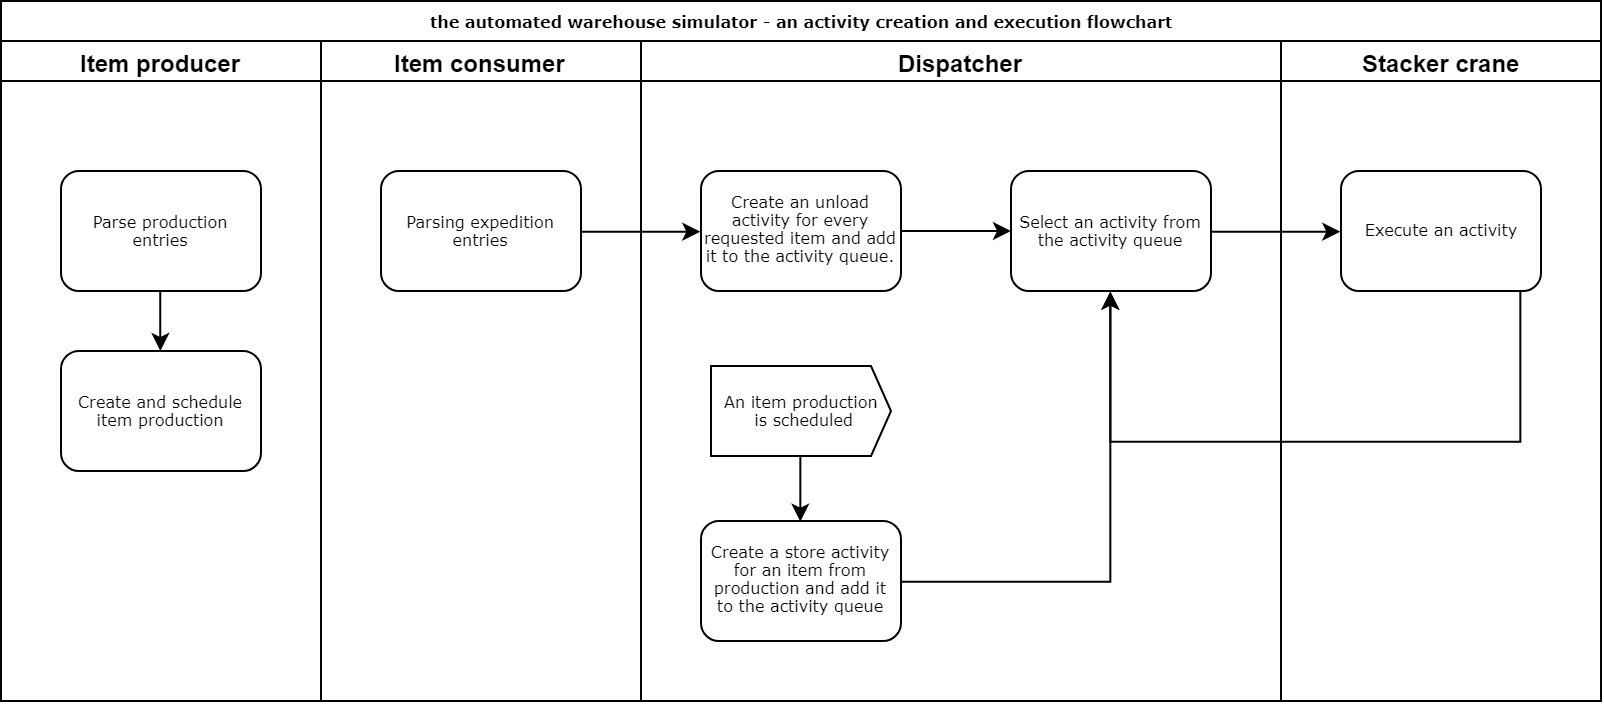
\includegraphics[width=1\linewidth]{flowchart2.png}
\caption{Diagram showing the flow of the activity creation and execution}
\label{flowchart1}
\end{figure}

\subsection{Activities}

Stacker cranes can pick up or put down an item, and move horizontally or vertically in an aisle. These actions are in the simulator wrapped into storing and unloading action.

\subsubsection{Stacker crane store activity}

Every SCS activity is associated with a stacker crane, an item to be stored and storage space to which it is going to be stored.

By executing this activity, a stacker crane carries out these actions.

\begin{enumerate}
    \item Move to the beginning of the aisle
    \item Pick up the item
    \item Move to the free position
    \item Store the item
\end{enumerate}

\subsubsection{Stacker crane unload activity}

Every SCU activity is associated with a stacker crane and an item to be unloaded.

By executing this activity, a stacker crane carries out these actions.

\begin{enumerate}
    \item Move to the item to be unloaded
    \item Pick up the item
    \item Move to the beginning of the aisle
    \item Put the item on the conveyor leading to expedition ramps
\end{enumerate}

\subsubsection{The activity queues}
\label{subsec:activityqueue}

 The activity queue stores activities to be executed. There are two activity queues. The first activity queue stores SCS activities and the second stores SCU activities. Both SCU and SCS activities are placed into their queues on creation. The way that activities are taken out and executed from the queue is shown in Pseudocode \ref{alg:activityexec}.

\begin{algorithm}[H]
\SetAlgoLined
{
\ForEach{$activity \leftarrow activityQueueSCS$}{
    \If{activity.stackerCrane is not idle}{
        $activity.execute()\;$
    }
}
\ForEach{$activity \leftarrow activityQueueSCU$}{
    \If{activity.stackerCrane is not idle}{
        $activity.execute()\;$
    }
}
}
\caption{Activity execution}
\label{alg:activityexec}
\end{algorithm}

The \emph{Activity execution} is triggered after activities creation or an activity is executed (Shown in Figure \ref{flowchart1}).


\subsection{Production and expedition handling in the simulator}

First off, the input of the simulator is config file describing the layout of the warehouse and stacker cranes parameters, csv file with item descriptors and time stamps representing the production schedule and csv file with an item types, quantities and truck id representing an expedition to be scheduled. To be clear what information is available, see Section \ref{subsubsubsec:availableinformation}.

Knowing what are activities and that we have files specifying production schedule and expedition demand, we describe how are these activities created and executed.

Starting with production, the schedule for the production is created at the beginning of a day in the simulation. Entries from the production input file are parsed and $PRODUCTION_GENERATED$ events put in the event queue. These events signalize that an item is produced and is on it's way to the automated warehouse. The dispatcher handles these events and decides to what aisle will the produced item be delivered and schedules a new event, $ITEM_ARRIVAL$, for the time it arrives to the assigned aisle. When the dispatcher handles $ITEM_ARRIVAL$ event, it creates SCS activity and puts it into the activity queue. How are activities executed from the activity queue is explained in Section \ref{subsubsec:activityqueue}.

The expedition handling works similarly, but it also has some major differences. The expedition input file is also parsed at the beginning of a day in the simulation. Then one event, $TRUCK\_ARRIVAL$, per expedition ramp are created (if there are more trucks planned for that day than expedition ramps) and they are scheduled for the beginning of the work hours. 

The dispatcher creates SCU activities from a truck expedition request upon catching $TRUCK\_ARRIVAL$ event. After every SCU activity of a truck expedition is finished, another $TRUCK\_ARRIVAL$ event is trigger for some another planned truck for that day.  

Order at which trucks are called or activities are processed is random.

The simulator generates report at the end, which includes information about truck expedition durations, time stamps of activities, reached buffer sizes, average idle times of stacker crane among other.

\section{Scheduler module}

In this section, we will describe integration into the simulator first and then we describe the implementation of the algorithm itself.

\subsection{The simulator integration}

*

\subsection{Algorithm implementation}

The following described the details of the implementation the algorithm from Chapter \ref{ch:Proposed solution}. The first phase, truck allocation, was solved using open-source constraint programming library, ***

\subsubsection{Truck allocation}

As proposed in Section \ref{sec:truckallocationprop}, the truck allocation is solved using Constraint programming. Specifically, I used Choco open-source java library dedicated to constraint programming \cite{choco}. The library can be used to model the problem in declarative way by stating the set of constraints. The library comes up with many different constraints with state-of-the-art implementations, offers different search algorithms and strategies and also provide multi-thread resolution. The scheduler is able to achieve good performance and allows the developer to easily tweak or modify the solving process.

\subsubsection{Job dispatching}

*uml

\subsubsection{Re-ordering and Idle time insertion}

opta


\chapter{Evaluation}
\label{ch:Evaluation}
\section{Performance}
\section{Scenarios}
Quickly summarize data 
\section{Comparison}
\subsection{Comparison of plan and behavior in simulation}
Comparing different version (LS, no LS, heuristic 1, heuristic 2, ...) of algorithm too.
\subsection{Effect of objectives?}
Mainly significance of idle times (at scanner or machines)
\chapter{Conclusion}

\bibliographystyle{plain}
\bibliography{refs.bib}



*************************

 and sorts them by their execution time (Since SCS activities do not have specified execution time, they are always prioritized and placed at the beginning the queue sorted from FIFO order)
 
 

Having a feasible schedule, we know how long it is, and we can tell approximately how much time we have until work hours end. We can take this time a distribute it in between items as idle times. We cannot simply determine where or how big idle times we should insert, because inserting an idle time in between some items may not result in a feasible schedule. We have to run step 2 of the algorithm, job dispatching, again after any insertion of idle times.


\label{overlap}
\begin{algorithm}[H]
\SetAlgoLined
\SetKwInOut{Input}{input}\SetKwInOut{Output}{output}
\Input{$c_i$ - completion time of an item $i$, $c_j$ - completion time of an item $j$, $r_i$ ramp to which item $i$ is assigned, $r_j$ ramp to which an item $j$ is assigned\\}
\Output{$1$ - Process of unloading items $i$ and $j$ does not overlap, $0$ - Process of unloading items $i$ and $j$ overlaps either at stacker crane, scanner or a conveyor}

$s_i = c_i - s\;$\\
$s_j = c_j - s\;$\\
$scc_i = s_i - t_{r_i}\;$\\
$scc_j = s_j - t_{r_j}\;$\\

$scs_i = scc_i - p_i\;$\\
$scs_j = scc_j - p_j\;$

\If{$m_i = m_j$}{
    \If{$scc_i > scs_j \land scc_j > scs_i$}{
        return $0\;$ \tcc{Processing of an items $i$ and $j$ is overlapping at stacker crane $m_i$}
    }
}

\If{$r_i = r_j$}{
    \If{$c_i  + \theta_i > s_j \land c_j + \theta_j > s_i$}{
        return $0\;$ \tcc{Processing of an items $i$ and $j$ is overlapping at expedition ramp $r_i$}
    }
}

return $1\;$
 \caption{Constraint - noOverlap}
\end{algorithm}

Alternatively, we can formulate this problem (with single expedition ramp) as a linear program, as follows:\\
\textbf{Decision variables}

\begin{itemize}
\item $x_{ij}$: 1 if $job_i$ expedited immediately after $job_j$, 0 otherwise
\item$c_i$: completion time of $job_i$ on the second stage
\item$idle_i$: idle time followed after $job_i$ on the second stage
\item$y_i$: order number of $job_i$ on the second stage
\item$scc_i$: start time of $job_i$ on the first stage 
\end{itemize}
\textbf{Data}
\begin{itemize}
\item$p_i$: processing time of $job_i$ on the first stage
\item$E_i$: set of allowed order numbers on the second stage for $job_i$
\item$I_i$: set of indexes of jobs scheduled on machine $i$ on the first stage
\item$M$: represents a large number
\item$start$: time at which work hours start
\item$end$: time at which work hours end
\end{itemize}

\begin{equation}
\begin{aligned}
&\text{minimize}
&&f(\ldots)
\end{aligned}
\end{equation}
\begin{equation}
\begin{aligned}
\text{subject to}\\
& \sum_{i=0}^{n} x_{ij} = 1 &&\\
& c_{i} - c_{j} + M(1 - x_{ij}) \geq s + idle_{i} && \text{for}\; i,j = 1, \ldots, n\\
& c_{i} - scc_{i0} = p_{i} + t_i + s + idle_i && \text{for}\; i = 1, \ldots, n\\
& scc_{i} + p_i < scc_j + M(1 - x_{ij}) && k = 0,\ldots,n, i,j \in I_k\\
& y_{i} - y_{j} < c_i - c_j + M(1 - x_{ij}) && \text{for}\; i,j = 1, \ldots, n\\
& y_i \in E_i && \text{for}\; i = 1, \ldots, n\\
& x_{ij} \in \{0, 1\}  && \text{for}\; i,j = 1, \ldots, n\\ 
& c_i \geq start && \text{for}\; i = 1, \ldots, n\\
& c_i \leq end && \text{for}\; i = 1, \ldots, n\\
& scc_{i} \geq start - p_i && \text{for}\; i = 1, \ldots, n\\
& idle_i \geq 0 && \text{for}\; i = 1, \ldots, n\\
\end{aligned}
\end{equation}
\\


\end{document}

